
\begin{wrapfigure}{r}{0.2\textwidth}
  \centering
  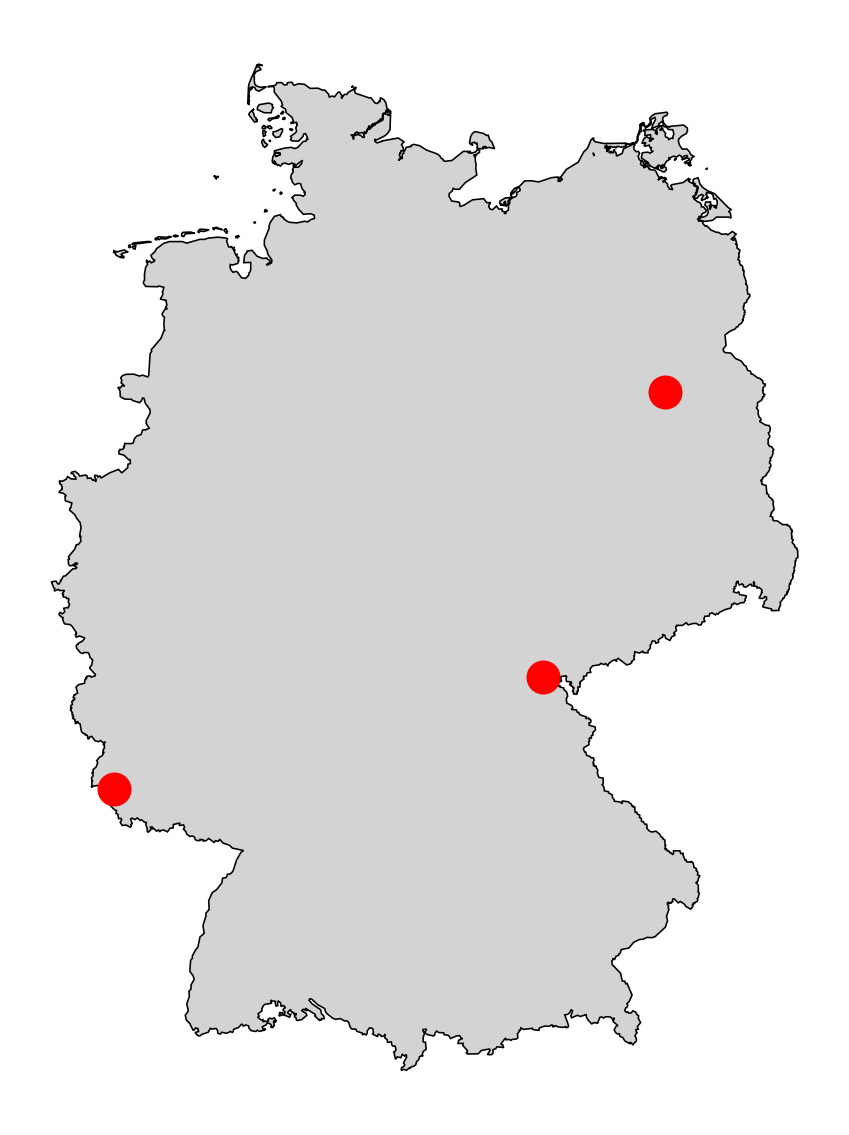
\includegraphics[width=0.18\textwidth]{deutschlandkarte.png}
\end{wrapfigure}

Das Coasterbot Team ist bei Stichprobengröße $N=3$ in guter Näherung über ganz Deutschland verteilt und die Kommunikation fand folglich komplett digital statt. Die Teamleitung und Kommunikation in den Meilensteingesprächen wurde durch Dennis Borutta wahrgenommen. Die Aufgaben wurden in Arbeitspakete auf- und im Team verteilt. Ein wöchentliches Meeting wurde per Videokonferenz durchgeführt, in denen jedes Teammitglied Fortschritte mitgeteilt, auf eventuelle Probleme hingewiesen sowie um eventuelle Hilfe gebeten hat. Kurze Rückmeldungen dazwischen wurden in der Woche über eine WhatsApp-Gruppe geteilt. In der Kommunikation traten keine Probleme auf. 


\subsubsection*{Projektverwaltung: Notion}

\begin{wrapfigure}{r}{0.6\textwidth}
  \centering
  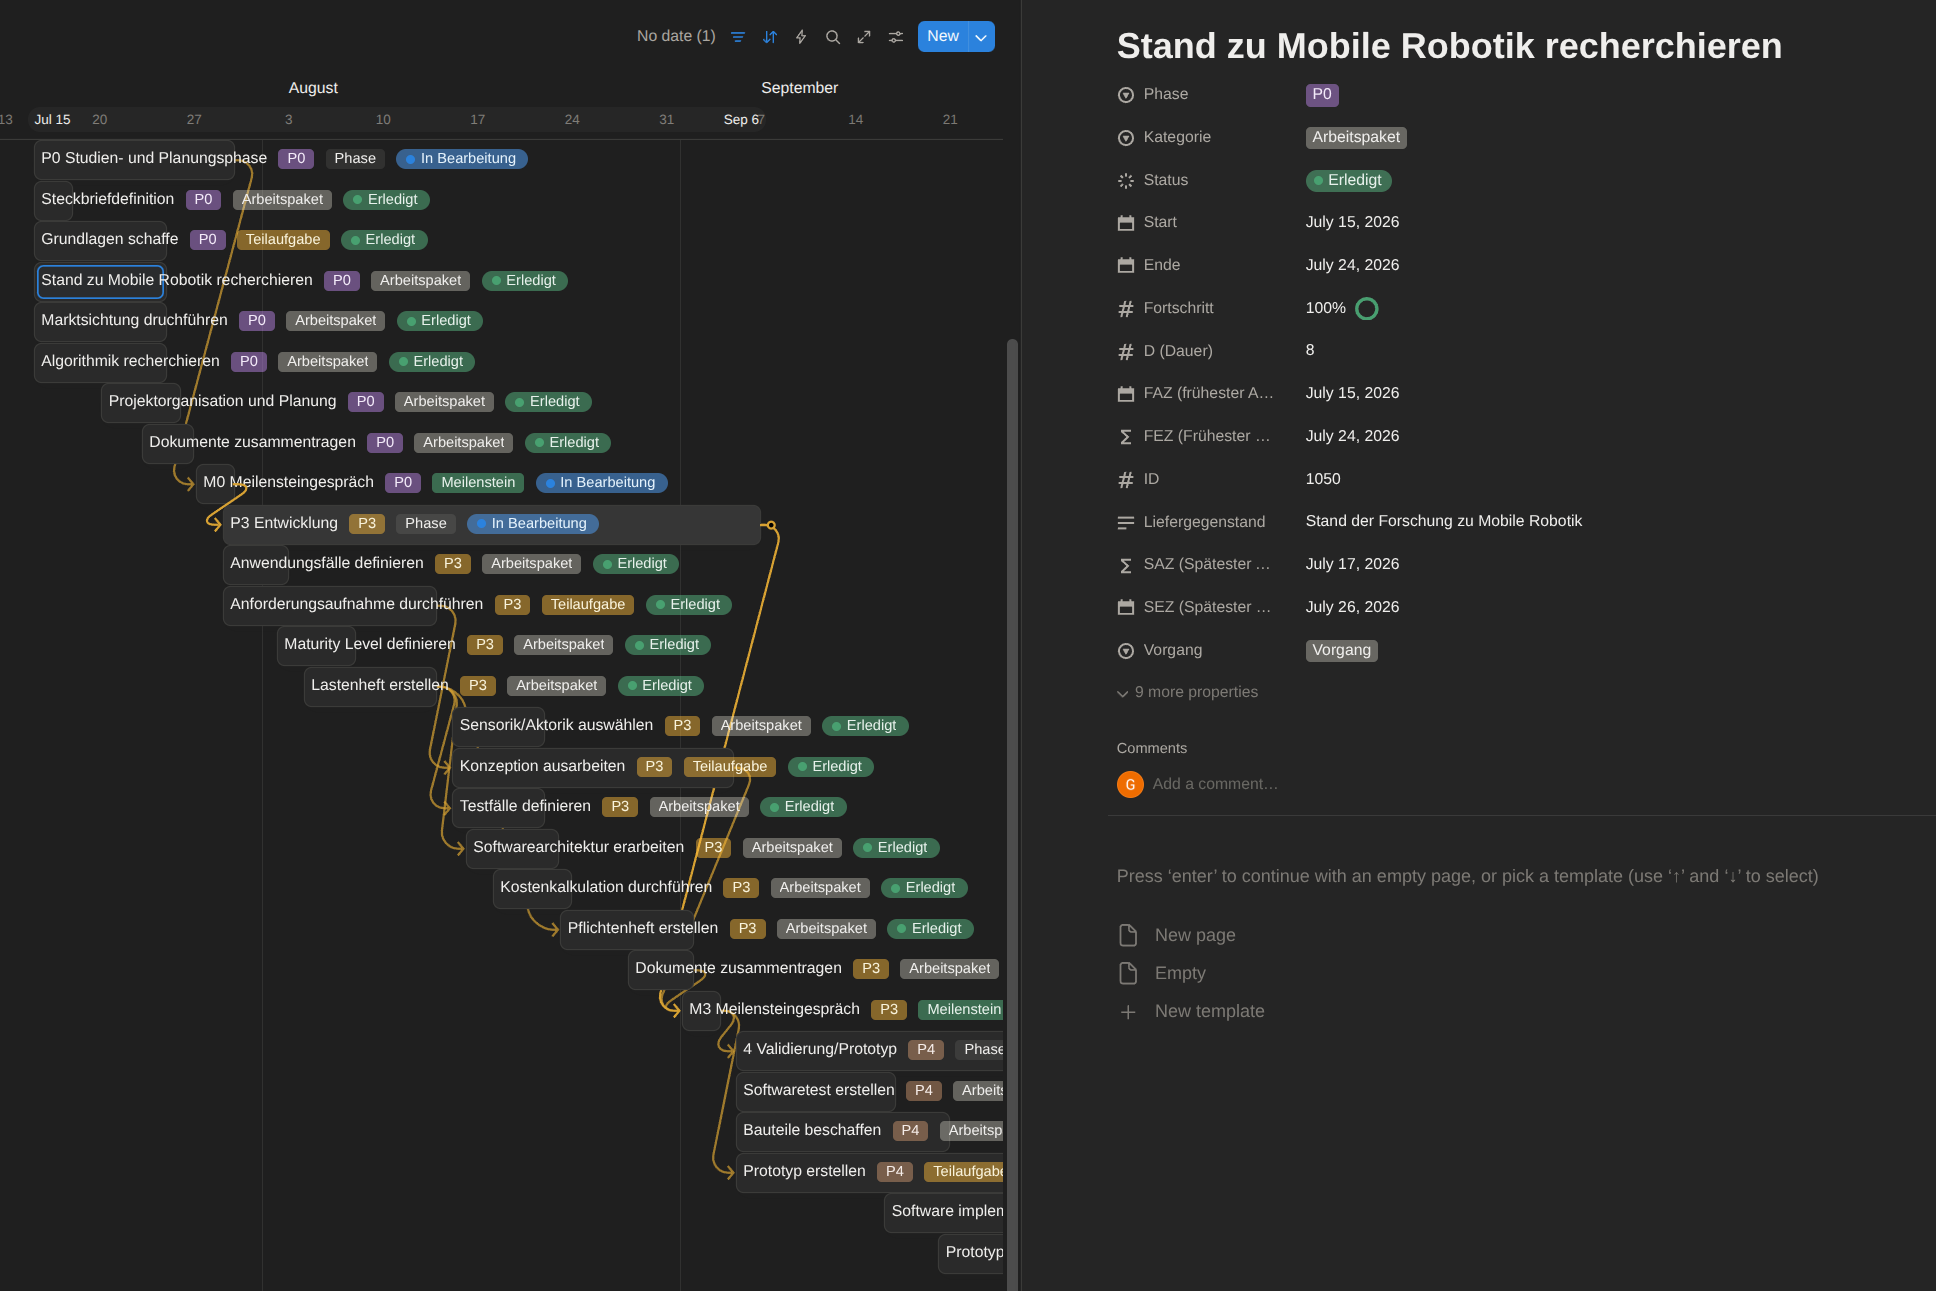
\includegraphics[width=0.58\textwidth]{notion_screenshot.png}
\end{wrapfigure}

Das Zentrale Projektsteuerungstool war \textbf{Notion}\footnote{\url{https://www.notion.com}}. Dieses wurde zur Bestimmung von Verantwortlichkeiten, Unteraufgaben, Deadlines und Terminen genutzt, hauptsächlich gepflegt durch Dennis Borutta. Es ermöglicht neben einer wie der rechts dargestellten Timelinedarstellung auch ein kollaboratives Dokumentenmanagement, welches durch das Team insbesondere in der Anfangsphase des Projekts für Recherche und Brainstorming genutzt wurde. 


\subsubsection*{Kollaborationsplatform: Github}

Das Projekt inklusive aller in \LaTeX\, erstellten Dokumente, Sourcecode und anderer Entwicklungsdateien sind in einem Github\footnote{\url{https://github.com}} Projekt verfügbar\footnote{\url{https://github.com/Project-CoasterBot/coasterbot}}. Git\footnote{\url{https://git-scm.com}} ist ein Versionsverwaltungssystem für das dezentrale Verwalten verschiedener Versionsstände und ist für das Coasterbot Projekt gewählt worden weil das Team bereits vertraut mit diesem Tool war, es kostenlos und Cross-Platform verfügbar ist. Github ist wiederum die zentrale Platform, an dem die Versionsstände wiederum gehostet werden. 


\subsubsection*{Videokonferenz: Alfaview}

Als Videokonferenzsystem für den wöchentlichen Austausch wurde auf eine Lösung der deutschen Firma Alfaview\footnote{\url{https://alfaview.com}} aus Karlsruhe gesetzt. Es ermöglicht neben regulärer Videokonferenz sowohl das Teilen von Dateien als auch ein Screensharing, was für den Austausch der Arbeitsstände enorm vorteilhaft war. 

\subsubsection*{Kommunikation: WhatsApp}

Für schnelle informelle Abstimmung und Terminabsprachen wurde der Instant-Messanging WhatsApp\footnote{\url{https://whatsapp.com}} genutzt. Die Kommunikation erfolgte hier aufgrund der unterschiedlichen Berufsauslastung und familärer Situation im Team asynchron. 

